\documentclass[aspectratio=169]{beamer}
\usetheme{Madrid}
\usepackage[T1]{fontenc}
\usepackage[utf8]{inputenc}
\usepackage[spanish,es-nodecimaldot]{babel}
\usepackage{amsmath}
\usepackage{booktabs}
\usepackage{graphicx}
\usepackage{tikz}
\usetikzlibrary{positioning,arrows.meta}

\graphicspath{{figures/pulsedb/}{./}}

\title{Proyecto AASIM}
\subtitle{Fase 2: Preparación de datos, gobernanza y validez (resultados sobre PulseDB v2.0)}
\author[Equipo E]{Equipo E (Juan Manuel Buitrago, Luis Carlos Rocha, German Alberto Hidalgo)}
\date{\today}

\definecolor{aasimazul}{HTML}{1F4E8C}
\definecolor{aasimrojo}{HTML}{B3261E}
\definecolor{aasimverde}{HTML}{1B7F3B}
\newcommand{\cumple}{\textcolor{aasimverde}{\textbf{Cumple}}}
\newcommand{\nocumple}{\textcolor{aasimrojo}{\textbf{No cumple}}}
\newcommand{\parcial}{\textcolor{aasimazul}{\textbf{Parcial}}}

\begin{document}

\begin{frame}
  \titlepage
\end{frame}

% ---------------------------------------------------------------
\begin{frame}{Objetivo, entregables y alcance}
  \textbf{Objetivo:} dejar los datos de ECG y presión arterial listos, trazables y libres de fuga
  de información antes de entrenar modelos en la Fase 3.

  \vspace{0.5em}
  \begin{columns}[T]
    \begin{column}{0.50\textwidth}
      \textbf{Entregables}
      \begin{enumerate}
        \item Data Quality Report (DQR)
        \item Diccionario de datos y esquema de metadatos
        \item Lista y matriz de riesgos de validez
        \item Pipeline modular de preprocesamiento
      \end{enumerate}
    \end{column}
    \begin{column}{0.46\textwidth}
      \textbf{Responsables}
      \begin{itemize}
        \item \textbf{Buitrago:} validación clínica y comparadores
        \item \textbf{Rocha:} señales, características y particiones
        \item \textbf{Hidalgo:} privacidad, equidad y calidad de señal
      \end{itemize}
    \end{column}
  \end{columns}

  \vspace{0.5em}
  \begin{block}{Alcance de los resultados}
    El corpus real es \textbf{PulseDB v2.0} (MIMIC-III y VitalDB). Las etiquetas se
    caracterizaron completas (5\,361 sujetos); las formas de onda, sobre una
    \textbf{muestra} de 41 sujetos y 2\,042 ventanas. Es un diagnóstico preliminar,
    no desempeño clínico.
  \end{block}
\end{frame}

% ---------------------------------------------------------------
\begin{frame}{Pipeline de preprocesamiento}
  \centering
  \begin{tikzpicture}[
      node distance=6mm,
      caja/.style={draw=aasimazul, rounded corners, fill=aasimazul!8, align=center,
                   minimum width=2.3cm, minimum height=1.3cm, font=\footnotesize},
      flecha/.style={-{Stealth}, thick, color=aasimazul}]
    \node[caja] (a) {ECG crudo\\ + etiquetas PA};
    \node[caja, right=of a] (b) {Filtros\\ causales\\ (RF1, R1)};
    \node[caja, right=of b] (c) {Compuerta\\ SQI\\ (RF4, R4)};
    \node[caja, right=of c] (d) {65\\ características};
    \node[caja, right=of d] (e) {Partición\\ por paciente\\ y centro};
    \draw[flecha] (a) -- (b);
    \draw[flecha] (b) -- (c);
    \draw[flecha] (c) -- (d);
    \draw[flecha] (d) -- (e);
  \end{tikzpicture}

  \vspace{0.8em}
  \begin{itemize}
    \item \textbf{Filtrado:} pasa-altos Butterworth (0.5 Hz), notch adaptativo a 50/60 Hz con $Q\ge 35$
          y pasa-bajos (45 Hz), todo causal y con estado; el modo de fase cero se rechaza en inferencia.
    \item \textbf{Muestreo:} PulseDB entrega ECG a 125 Hz; el mínimo del esquema se ajustó de 250 a 125 Hz
          (riesgo V-18: resolución de 8 ms por muestra).
    \item \textbf{Etiquetas:} censura clínica de PAS fuera de 70--240 mmHg, PAD fuera de 40--140 mmHg
          y presión de pulso menor de 20 mmHg.
  \end{itemize}
\end{frame}

% ---------------------------------------------------------------
\begin{frame}{El corpus: PulseDB v2.0}
  \begin{columns}[T]
    \begin{column}{0.52\textwidth}
      \small
      \begin{tabular}{lrr}
        \toprule
        & MIMIC & VitalDB \\
        \midrule
        Sujetos & 2\,423 & 2\,938 \\
        Segmentos (10 s, 125 Hz) & 3\,791\,004 & 1\,454\,450 \\
        Edad media (adultos) & 63.5 & 59.2 \\
        Mujeres & 42 \% & 45 \% \\
        IMC disponible & 0 \% & 100 \% \\
        Etiquetas censuradas & 3.56 \% & 1.88 \% \\
        \bottomrule
      \end{tabular}

      \vspace{0.6em}
      Adultos: 5\,332; 43.5 \% con 65 años o más.
    \end{column}
    \begin{column}{0.44\textwidth}
      \begin{block}{Límites que condicionan el uso}
        \small
        \begin{itemize}
          \item Población hospitalaria con catéter arterial.
          \item Sin postura, medicación ni comorbilidades.
          \item Solo dos centros.
          \item Licencias ODbL y CC BY-NC-SA 4.0: revisión legal antes de uso comercial.
        \end{itemize}
      \end{block}
    \end{column}
  \end{columns}
\end{frame}

% ---------------------------------------------------------------
\begin{frame}{Cuotas ISO 81060-2 en las etiquetas}
  \begin{columns}[c]
    \begin{column}{0.60\textwidth}
      \centering
      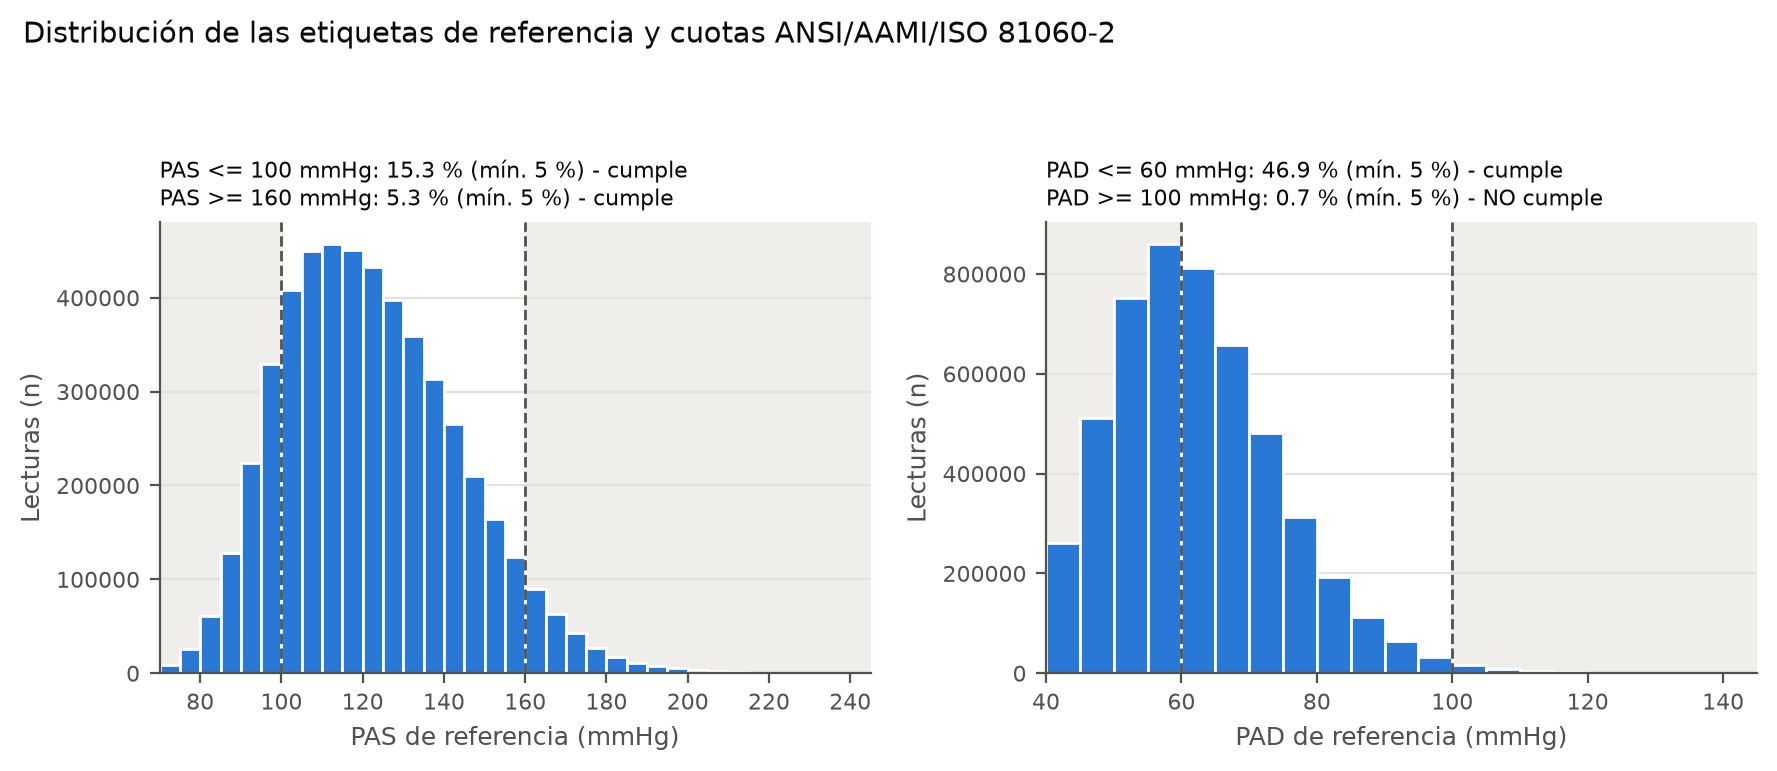
\includegraphics[width=\linewidth,height=0.60\textheight,keepaspectratio]{histograma_pas_pad_pulsedb.png}
    \end{column}
    \begin{column}{0.38\textwidth}
      \small
      \begin{tabular}{lrc}
        \toprule
        Rango & Fracción & \\
        \midrule
        PAS $\le$ 100 & 15.3 \% & \cumple \\
        PAS $\ge$ 160 & 5.3 \% & \cumple \\
        PAD $\le$ 60 & 46.9 \% & \cumple \\
        PAD $\ge$ 100 & 0.65 \% & \nocumple \\
        \bottomrule
      \end{tabular}

      \vspace{0.4em}
      \footnotesize
      Mínimo exigido: 5 \%. VitalDB por sí sola no cumple PAS $\ge$ 160 (1.9 \%);
      en la partición de prueba, PAS $\ge$ 160 baja a 4.7 \%.
      \alert{El desempeño en la cola diastólica alta no podrá afirmarse.}
    \end{column}
  \end{columns}
\end{frame}

% ---------------------------------------------------------------
\begin{frame}{Sincronización ECG--referencia (supuesto S3)}
  \begin{columns}[c]
    \begin{column}{0.60\textwidth}
      \centering
      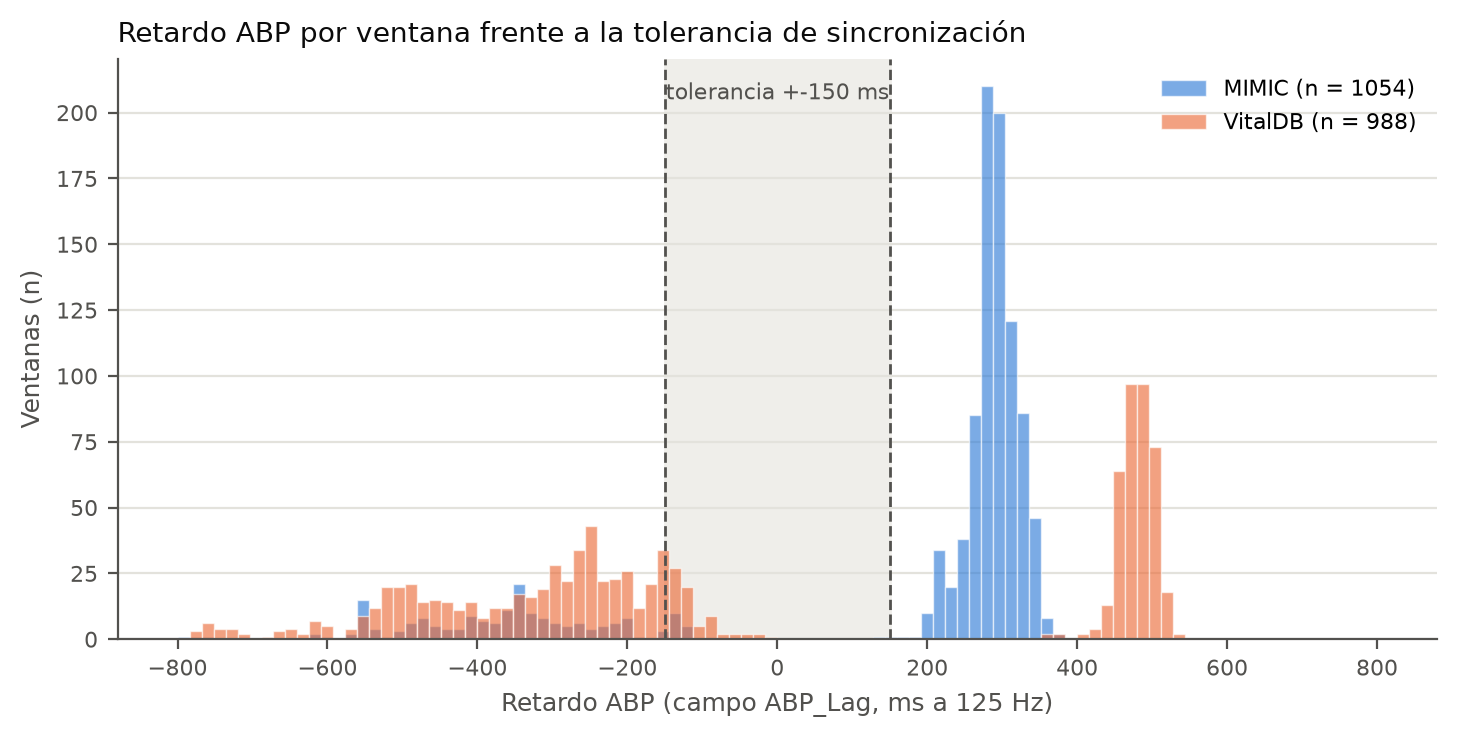
\includegraphics[width=\linewidth,height=0.60\textheight,keepaspectratio]{retardo_abp_pulsedb.png}
    \end{column}
    \begin{column}{0.38\textwidth}
      \small
      \begin{itemize}
        \item Desfase de alineación \texttt{ABP\_Lag} de PulseDB: mediana $+280$ ms (MIMIC)
              y $-176$ ms (VitalDB).
        \item \textbf{99.7 \%} de las ventanas superan la tolerancia de 50 ms.
        \item El signo cambia dentro de un mismo sujeto en el 27 \% de las ventanas consecutivas.
      \end{itemize}
      \vspace{0.3em}
      \alert{La fuente no garantiza S3.} Falta confirmar la definición exacta del campo con la
      documentación de la base.
    \end{column}
  \end{columns}
\end{frame}

% ---------------------------------------------------------------
\begin{frame}{Compuerta de calidad de señal (RF4) con datos reales}
  \begin{columns}[T]
    \begin{column}{0.48\textwidth}
      \small
      Umbrales del plan: bSQI $\ge 0.85$, kSQI $\ge 5.0$, pSQI $\ge 0.50$.

      \vspace{0.4em}
      \begin{tabular}{lrr}
        \toprule
        Muestra (2\,042 ventanas) & n & \% \\
        \midrule
        Retenidas & 1\,109 & 54.3 \\
        Rechazadas & 933 & 45.7 \\
        \quad por bSQI & 77 & 3.8 \\
        \quad por kSQI & 131 & 6.4 \\
        \quad por pSQI & 927 & 45.4 \\
        \bottomrule
      \end{tabular}

      \vspace{0.4em}
      Mediana de pSQI: 0.52 (MIMIC) y 0.50 (VitalDB): el umbral cae sobre la mediana.
    \end{column}
    \begin{column}{0.48\textwidth}
      \small
      \textbf{Sensibilidad exploratoria del umbral de pSQI}

      \begin{tabular}{crrrr}
        \toprule
        pSQI & Global & 18--64 & $\ge$65 & Cociente \\
        \midrule
        0.50 & 45.7 & 35.0 & 70.8 & 2.0 \\
        0.40 & 22.8 & 12.8 & 46.5 & 3.6 \\
        0.30 & 13.2 & 4.7 & 33.2 & 7.1 \\
        \bottomrule
      \end{tabular}

      \vspace{0.4em}
      \alert{Hallazgo:} bajar el umbral reduce la pérdida, pero aumenta la disparidad por edad.
      El pSQI mide morfología correlacionada con la edad y debe rediseñarse; los umbrales no se
      congelan con esta muestra.
    \end{column}
  \end{columns}
\end{frame}

% ---------------------------------------------------------------
\begin{frame}{Rechazo selectivo por subgrupo (riesgo V-09)}
  \begin{columns}[c]
    \begin{column}{0.60\textwidth}
      \centering
      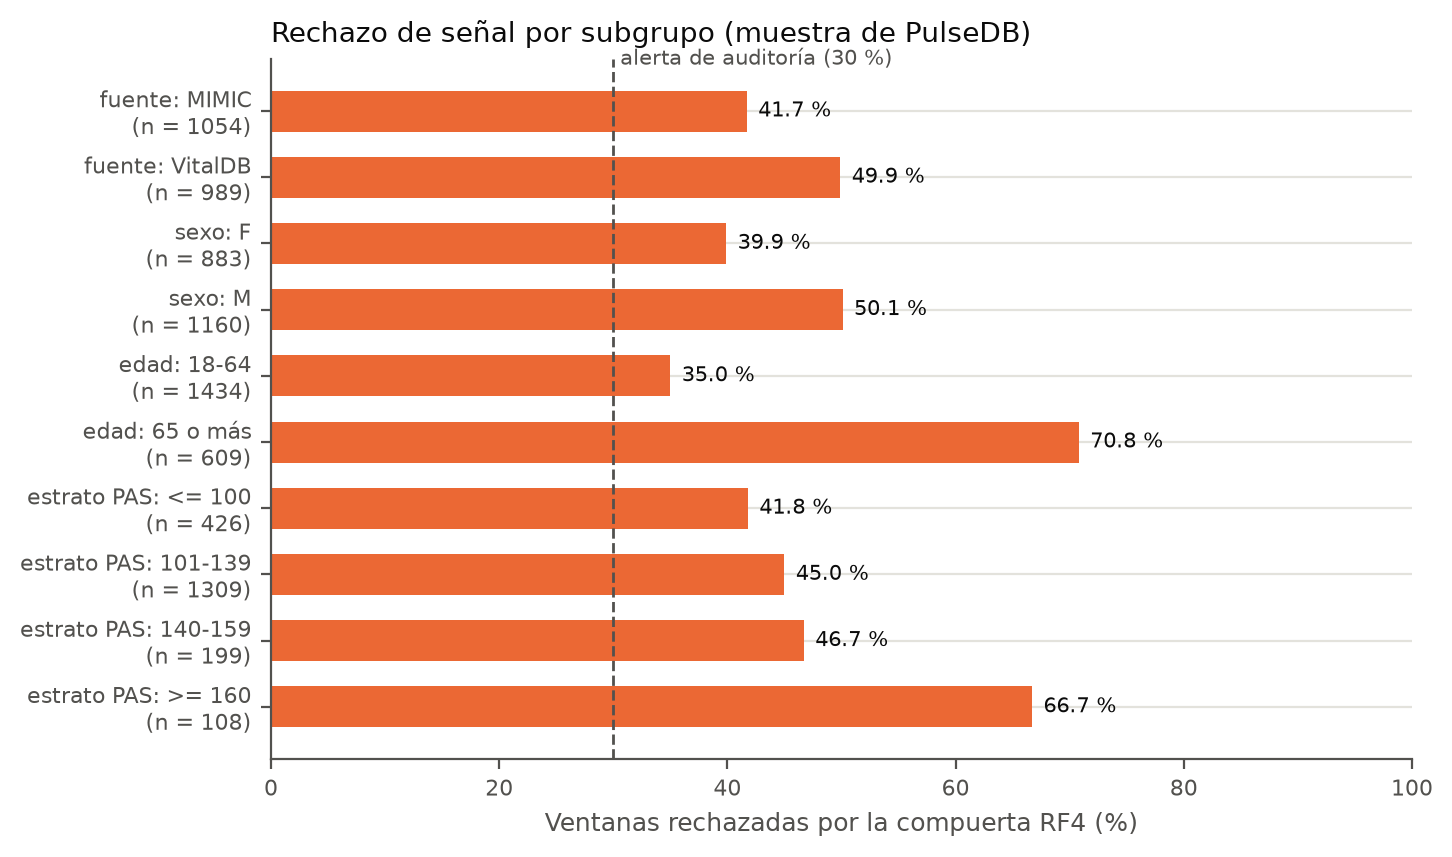
\includegraphics[width=\linewidth,height=0.64\textheight,keepaspectratio]{rechazo_por_subgrupo_pulsedb.png}
    \end{column}
    \begin{column}{0.38\textwidth}
      \small
      \begin{itemize}
        \item Edad: 35.0 \% (18--64) frente a 70.8 \% (65 o más); cociente \textbf{2.02}.
        \item Estrato de PAS: 41.8 \% ($\le$100) a 67.3 \% ($\ge$160); cociente \textbf{1.61}.
        \item Sexo 1.26; fuente 1.20.
      \end{itemize}
      \vspace{0.3em}
      Criterio de la puerta G8: cociente $\le 1.5$. \nocumple

      \vspace{0.3em}
      \footnotesize
      Pérdida neta en la muestra: 46.7 \% (criterio $<15$ \%). Celdas con menos de 5 sujetos
      agrupadas.
    \end{column}
  \end{columns}
\end{frame}

% ---------------------------------------------------------------
\begin{frame}{Características y latencia sobre ventanas reales}
  \begin{columns}[T]
    \begin{column}{0.56\textwidth}
      \small
      \begin{itemize}
        \item 65 características por ventana: morfología, HRV, wavelet Daubechies 4 y textura GLCM.
        \item QRS $90\pm15$ ms, coherente; PR satura en 264 ms en el 6.5 \% de las ventanas;
              QT y QTc con dispersión alta: a 125 Hz son de \textbf{baja fiabilidad}.
        \item Entropía muestral indefinida en 39.8 \% de las ventanas; VLF constante en 10 s.
        \item Correlación máxima con la presión: $|\rho| = 0.37$ (textura y amplitud del QRS),
              con posible confusión por ganancia y electrodo.
        \item Detector de picos R: F1 = 1.00 (mediana) frente a las anotaciones de PulseDB.
      \end{itemize}
    \end{column}
    \begin{column}{0.40\textwidth}
      \begin{block}{Latencia (RNF2)}
        \small
        2\,041 ventanas reales de 10 s en el equipo de trabajo (2 CPU):
        media 12.5 ms, percentil 99 43.4 ms, máximo 93.8 ms; margen mínimo de 53 veces
        frente a 5 s. Se repetirá en el hardware de referencia.
      \end{block}
      \begin{block}{Interferencia de red}
        \small
        Detectada en 34--42 \% de las ventanas; el detector marca 50 Hz en VitalDB donde se
        esperaba 60 Hz: pendiente de verificación.
      \end{block}
    \end{column}
  \end{columns}
\end{frame}

% ---------------------------------------------------------------
\begin{frame}{Particionamiento sin fuga y privacidad}
  \begin{columns}[T]
    \begin{column}{0.56\textwidth}
      \small
      \begin{tabular}{lrrr}
        \toprule
        Partición & Sujetos & MIMIC & VitalDB \\
        \midrule
        Entrenamiento & 3\,732 & 1\,695 & 2\,037 \\
        Validación & 800 & 363 & 437 \\
        Prueba & 800 & 363 & 437 \\
        \bottomrule
      \end{tabular}

      \vspace{0.5em}
      \begin{itemize}
        \item Estratificada por fuente, edad, sexo y PAS: edad media 61 años y 43.8 \% de mujeres
              en las tres particiones.
        \item \textbf{Certificado:} 0 sujetos y 0 huellas SHA-256 en común; manifiesto sellado.
        \item Con dos centros no cabe la partición por sitio 70/15/15: se usa
              \textit{leave-one-site-out}.
      \end{itemize}
    \end{column}
    \begin{column}{0.40\textwidth}
      \begin{block}{Privacidad (RNF1)}
        \small
        Identificadores opacos \texttt{SUBJ-xxxxx}; los nombres originales de PulseDB quedan
        en una tabla de acceso restringido; edad en rangos; celdas con $n<5$ agrupadas.
      \end{block}
      \begin{block}{Esquema de metadatos 1.1.0}
        \small
        ECG a 125 Hz o más; categorías \texttt{not\_available} para IMC y postura cuando la
        fuente no las aporta.
      \end{block}
    \end{column}
  \end{columns}
\end{frame}

% ---------------------------------------------------------------
\begin{frame}{Riesgos de validez: qué confirmaron los datos reales}
  \centering
  \footnotesize
  \begin{tabular}{p{4.6cm}p{6.6cm}p{2.4cm}}
    \toprule
    Riesgo & Evidencia con PulseDB & Estado \\
    \midrule
    Fuga por identidad (V-01) & Partición certificada, 0 intersecciones & Implementado \\
    Sesgo retrospectivo (V-02) & Cadena causal en todo el pipeline; 41 pruebas superadas & Implementado \\
    Colapso hacia la media (V-04) & PAD $\ge$ 100 mmHg: 0.65 \% de las lecturas & \textcolor{aasimrojo}{Crítico} \\
    Desalineación temporal (V-05) & 99.7 \% de ventanas con desfase $>$ 50 ms & \textcolor{aasimrojo}{Crítico} \\
    Rechazo selectivo (V-09) & Cociente 2.02 por edad y 1.61 por PAS & \textcolor{aasimrojo}{Alto} \\
    Umbrales mal calibrados (V-10) & pSQI = 0.50 sobre la mediana; 45.7 \% de rechazo & \textcolor{aasimrojo}{Crítico} \\
    Resolución a 125 Hz (V-18) & PR satura; QRS y $dV/dt$ con 8 ms por muestra & Alto \\
    Dominio y licencia (V-19) & Población hospitalaria; CC BY-NC-SA 4.0 & Alto \\
    \bottomrule
  \end{tabular}

  \vspace{0.6em}
  Total: 19 riesgos evaluados por probabilidad y severidad (informe de riesgos).
\end{frame}

% ---------------------------------------------------------------
\begin{frame}{Puertas de decisión hacia la Fase 3}
  \begin{columns}[T]
    \begin{column}{0.52\textwidth}
      \small
      \begin{tabular}{p{4.6cm}c}
        \toprule
        Puerta & Estado \\
        \midrule
        G1 DQR (pérdida, cuotas) & \nocumple \\
        G2 Aislamiento de particiones & \cumple \\
        G3 Latencia & \parcial \\
        G5 Comparador certificado & \nocumple \\
        G6 Sincronización & \nocumple \\
        G7 Representatividad & \parcial \\
        G8 Rechazo no selectivo & \nocumple \\
        G11 Política causal & \cumple \\
        \bottomrule
      \end{tabular}

      \vspace{0.3em}
      \footnotesize G4, G9 y G10 pendientes; G12 con protocolo implementado.
    \end{column}
    \begin{column}{0.44\textwidth}
      \begin{block}{Decisión del equipo}
        \small
        Con G1 y G5 sin cumplir, la Fase 3 \textbf{no queda autorizada}. Rutas propuestas:
        \begin{enumerate}
          \item Rediseñar el índice espectral y recalibrar con \textit{train} y \textit{val}.
          \item Acotar por acta una etapa exploratoria sobre datos públicos, sin
                afirmaciones clínicas.
          \item Incorporar un conjunto propio con comparador certificado y sincronización controlada.
        \end{enumerate}
      \end{block}
    \end{column}
  \end{columns}
\end{frame}

\end{document}
